% Drawing 127/01-5 -- folder 127, batch 01, archive page 14 (PDF page 15).
% Transcription: page de notes et de croquis au crayon, sans texte suivi ; elles accompagnent le Th.~1.4 (pages 3--4). Les éléments en sont donnés dans l'ordre de la page, sans chercher à les relier
% Kind: page of pencil notes and sketches. Method 2 (schematic redraw from the facsimile). Status: partial.
% Notes: Whole page in pencil. Drawn: the diagram at the top left (X supset U, the stroke f down to Y, Y - Y'; X' supset U' over Y' with a stroke and a bracket, an oblique stroke towards x~_1, x~ (stacked, with a small arrow), G', x~'; F, F_U -> G_U, F -> i_*(G_U), with the arrows F -> G and G -> i_*), the margin diagram x' in (T_alpha)_y' with its arrow down to y' and the curved stroke from it; the vertical stroke and the implication arrow in the middle; the circled "EGA IV 12.2."; the circled phrase of the counter-example (a long loop); the two long separating curves; the counter-example sketch at the bottom left (X -> Y birational, a vertical pencil stroke to its left, a curve crossing a line with a vertical strip and a small arc, a base line with two points) and the long vertical stroke right of it. Nodes placed once; the strokes of the top diagram are on the lines between the node points. Left out: the formulas of the page (all in the transcription), including the parenthesis "( => x_alpha in Ass G_y )", the long faint diagonal strokes across the left half, and the small x_alpha | Y next to "Ass G_U" (part of the formula there). Still differs: the hand is schematic; the counter-example sketch is a reading of faint strokes. Redrawn 2026-11-09 (issue 128): to check again.
% Coordinates: 1 unit = 1 mm = 1/100 of the crop width (bbox in page fractions: [0.05, 0.05, 0.97, 0.87]).
% Redrawn by Claude (claude-opus-5-5), issue #73, 2026-11-09; not checked by a human; not compiled (no TeX in the session).
% Rights: reproduces part of the work -- behind RENDER_TRANSCRIPTS, never published by itself.
\documentclass[tikz,border=3pt]{standalone}
\usepackage{amsmath,amssymb}
\usetikzlibrary{patterns,arrows.meta}
\tikzset{pencil/.style={black!45}, struck/.style={black!35}, mark/.style={circle,draw,inner sep=1.3pt}, pt/.style={circle,fill,inner sep=0.9pt}, opt/.style={circle,draw,fill=white,inner sep=1.1pt}}
\begin{document}
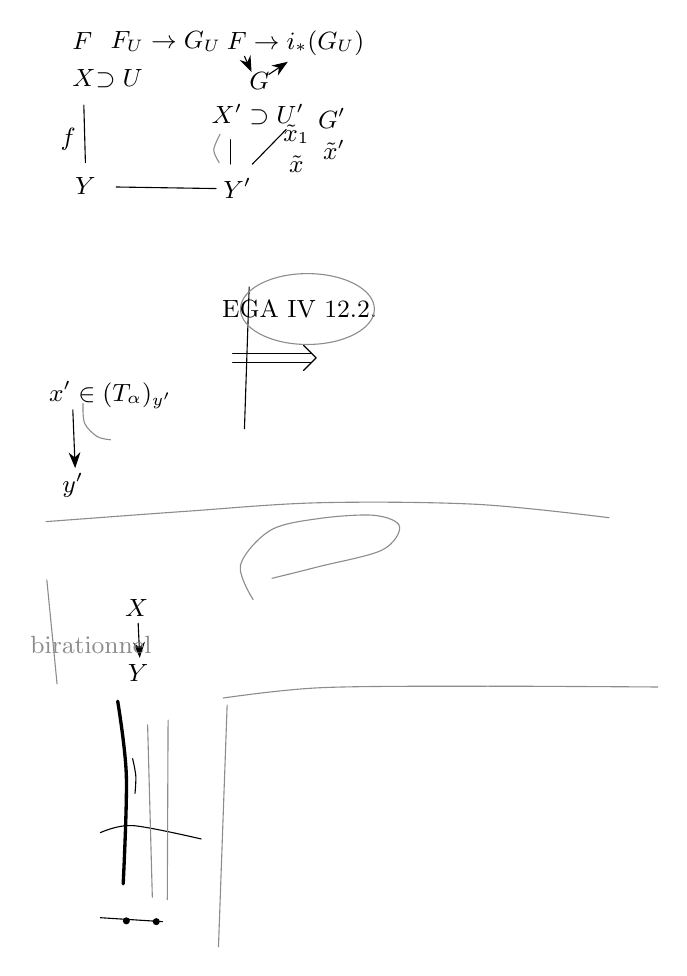
\begin{tikzpicture}[x=1mm,y=1mm,line cap=round,line join=round,font=\scriptsize]
\node[inner sep=1pt] at (20.1,-9.7) {\small $X$};
\node[inner sep=1pt] at (24.6,-9.7) {\small $\supset U$};
\node[inner sep=1pt] at (20.3,-23.4) {\small $Y$};
\node[inner sep=1pt] at (39.6,-23.7) {\small $Y'$};
\node[inner sep=1pt] at (18.1,-17.5) {\small $f$};
\draw (20.1,-13.1) -- (20.3,-20.4);
\draw (24.2,-23.5) -- (36.9,-23.7);
\node[inner sep=1pt] at (42.2,-14.3) {\small $X'\supset U'$};
\draw (38.7,-17.5) -- (38.7,-20.6);
\draw[pencil] plot[smooth, tension=0.55] coordinates {(37.4,-16.8) (36.6,-18.8) (37.3,-20.4)};
\draw (41.5,-20.6) -- (45.8,-16.2);
\node[inner sep=1pt] at (47.1,-16.8) {\small $\tilde{x}_1$};
\node[inner sep=1pt] at (47.1,-20.6) {\small $\tilde{x}$};
\node[inner sep=1pt] at (51.6,-14.8) {\small $G'$};
\node[inner sep=1pt] at (51.9,-18.8) {\small $\tilde{x}'$};
\node[inner sep=1pt] at (19.9,-5) {\small $F$};
\node[inner sep=1pt] at (30.5,-5) {\small $F_U\to G_U$};
\node[inner sep=1pt] at (47,-5.2) {\small $F\to i_*(G_U)$};
\draw[-{Stealth[length=2mm]}] (40.5,-6.9) -- (41.4,-8.9);
\node[inner sep=1pt] at (42.4,-10) {\small $G$};
\draw[-{Stealth[length=2mm]}] (43.6,-9.2) -- (46,-7.6);
\node[inner sep=1pt] at (23.5,-49.9) {\small $x'\in(T_\alpha)_{y'}$};
\draw[-{Stealth[length=2mm]}] (18.7,-51.8) -- (19,-59.2);
\node[inner sep=1pt] at (18.7,-61.4) {\small $y'$};
\draw[pencil] plot[smooth, tension=0.55] coordinates {(20,-51) (20.2,-53.5) (21.8,-55.2) (23.5,-55.6)};
\draw (41.1,-36.2) -- (40.5,-54.2);
\draw (39,-44.6) -- (49,-44.6);
\draw (39,-45.8) -- (49,-45.8);
\draw (48,-43.6) -- (49.6,-45.2) -- (48,-46.8);
\node[inner sep=1pt] at (47.5,-39) {\small EGA IV 12.2.};
\draw[pencil] (48.5,-39) ellipse[x radius=8.5, y radius=4.5];
\draw[pencil] plot[smooth, tension=0.55] coordinates {(15.3,-66) (32.9,-64.7) (50,-63.6) (70,-63.8) (86.8,-65.5)};
\draw[pencil] plot[smooth, tension=0.55] coordinates {(41.6,-75.9) (40,-71.5) (43.8,-67.1) (50,-65.6) (57,-65.2) (60.2,-66.6) (58,-69.6) (50,-71.7) (44,-73.2)};
\draw[pencil] plot[smooth, tension=0.55] coordinates {(37.8,-88.4) (50,-87.1) (70,-86.9) (93,-87)};
\node[inner sep=1pt] at (26.8,-77) {\small $X$};
\draw[-{Stealth[length=2mm]}] (27,-78.9) -- (27.2,-83.3);
\node[inner sep=1pt] at (27,-85.2) {\small $Y$};
\node[inner sep=1pt,pencil] at (21,-81.6) {\small birationnel};
\draw[pencil] (15.4,-73.4) -- (16.7,-86.6);
\draw[very thick] plot[smooth, tension=0.55] coordinates {(24.4,-88.8) (25.5,-98.3) (25.1,-112)};
\draw plot[smooth, tension=0.55] coordinates {(26.3,-96.1) (26.7,-98.3) (26.6,-100.5)};
\draw plot[smooth, tension=0.55] coordinates {(22.2,-105.5) (26.3,-104.6) (35,-106.3)};
\draw[pencil] (28.2,-91.8) -- (28.8,-113.7);
\draw[pencil] (30.8,-91.2) -- (30.7,-114);
\draw (22.2,-116.3) -- (30.1,-116.8);
\node[pt] at (25.5,-116.7) {};
\node[pt] at (29.3,-116.8) {};
\draw[pencil] (38.3,-89.3) -- (37.2,-120);
\end{tikzpicture}
\end{document}
